\chapter{Fehlerbehandlung}
\renewcommand{\chaptertitle}{Fehlerbehandlung}

\lehead[]{\sf\hspace*{-2.00cm}\textcolor{white}{\colorbox{lightblue}{\makebox[1.60cm][r]{\thechapter}}}\hspace{0.17cm}\textcolor{lightblue}{\chaptertitle}}
\rohead[]{\textcolor{lightblue}{\chaptertitle}\sf\hspace*{0.17cm}\textcolor{white}{\colorbox{lightblue}{\makebox[1.60cm][l]{\thechapter}}}\hspace{-2.00cm}}
%\chead[]{}
\rehead[]{\textcolor{lightblue}{AvHG, Inf, My}}
\lohead[]{\textcolor{lightblue}{AvHG, Inf, My}}

\lstset{style=myJava}

\section{Fehler-Klassen}

Informationen über aufgetretene Fehler werden in Java in Objekten der Klasse
\myClass{Exception} (oder einer abgeleiteten Klasse) transportiert. Das folgende
UML-Diagramm gibt einen Überblick über die Klassenhierarchie der Fehlermeldungen:

\begin{center}
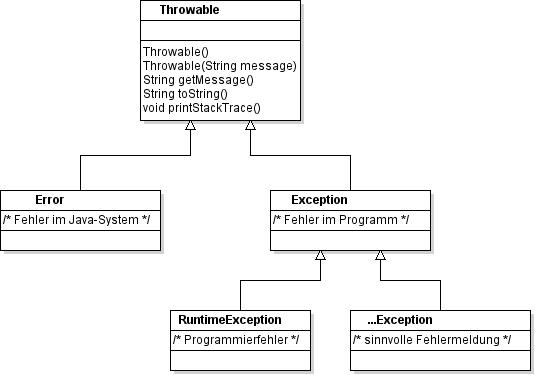
\includegraphics[width=0.9\textwidth]{./inf/SEKII/25_Java_Exceptions/ExceptionHierarchy.jpg}
\end{center}

\begin{compactitem}
\item Die Superklasse \textbf{\myClass{Throwable}} wird nie direkt verwendet.
\item \textbf{Errors} sind Fehler im System, die von den Programmierern des
Java-Systems verschuldet wurden. Normalerweise sollten niemals Errors auftreten.
\item \textbf{Exception} ist der Sammelbegriff für alle Fehler, die im Programm
behandelt werden können.
\item \textbf{RuntimeExceptions} sind Fehler, die durch falsche Programmierung
verursacht wurden (z.B. durch eine unerlaubte Typumwandlung). Bei korrekter
Programmierung dürfen RuntimeExceptions niemals auftreten.
\item \textbf{Sinnvolle Exceptions} (z.B. PrinterException – \glqq im Drucker
ist kein Papier\grqq ) sollten vom Programm abgefangen und dem Benutzer
angezeigt werden. Man kann auch eigene Exception-Klassen erzeugen.
\end{compactitem}

\subsection{Wichtige Methoden der Super-Klasse \myClass{Throwable}}

\bgroup
\def\arraystretch{1.2}
\begin{tabularx}{\textwidth}{|p{60mm}|X|}
\hline
\textbf{Methode} & \textbf{Erläuterung}
\\ \hline
\lstinline|Throwable()|\newline
\lstinline|Throwable(String message)| & 
Konstruktor: Es kann optional ein Fehlertext angegeben werden.
\\ \hline
\lstinline|String getMessage()| &
Liefert den Fehlertext zurück.
\\ \hline
\lstinline|String toString()| &
Liefert den Klassennamen der Exception und den Fehlertext zurück.
\\ \hline
\lstinline|public void printStackTrace()| &
Gibt auf der Konsole aus, bei welcher Programmzeile das Programm abgestürzt ist.
\\ \hline
\end{tabularx}
\egroup


\section{Beispiel}

\begin{compactenum}[a)]
\item \textbf{Erstellung einer eigenen Exception-Klasse}

\begin{lstlisting}
public class DurchNullException extends Exception {

    public DurchNullException() {
        super("Man kann nicht durch 0 teilen.");
    }

    public DurchNullException(String text) {
        super(text);
    }
}
\end{lstlisting}

\item \textbf{Exceptions auslösen (\lstinline|throw|)}

\begin{lstlisting}
æpublic class Formeln {

    public static double division(double x1, double x2) æthrows DurchNullExceptionæ { 
        if (x2 == 0) {
æ            DurchNullException fehler;
            fehler = new DurchNullException();
            throw fehler;
æ            // Oder kürzer:
            // throw new DurchNullException("Teilen durch 0 ist verboten!");
        }
        return (x1 / x2);
    }
}
\end{lstlisting}

Durch den Zusatz \lstinline|throws| im Methodenkopf, wird der Methode erlaubt
eine auftretende Exception der angegebenen Art an die aufrufende Methode weiter
zu reichen. Umgekehrt wird diese Information vom Java-System auch dazu benutzt
zu erkennen, dass durch den Aufruf dieser Methode eine entsprechende Exception
erzeugt werden kann (und dass in der aufrufenden Methode entsprechende
Maßnahmen zum Umgang mit dieser Exception getroffen werden müssen).

Der Befehl \lstinline|throw| im Methodenkörper schließlich löst diese Exception
dann aus.

\item \textbf{Exception abfangen (\lstinline|catch|)}

\begin{lstlisting}
public class ExceptionBsp {

æ    public static void main(final String[] args) {
æ        try {
æ            for (int i = 5; i > -5; i--) {
                System.out.println("10 durch " + i + " = "
                        + Formeln.division(10, i));
            }
æ        } catch (DurchNullException e) {
æ            System.out.println(æe.getMessage()æ);
        }
æ    }
}
\end{lstlisting}

Exceptions können in einem \lstinline|try-catch| Block abgefangen und behandelt
werden. Im \lstinline|try| Teil dieses Konstrukts steht der Teil des Codes, in
dem eine Exception auftreten kann.

Für den Fall, dass die Exception tatsächlich ausgelöst wird, werden alle
noch folgenden Befehle innerhalb des \lstinline|try|-Blocks übersprungen und
statt dessen, die Befehle im \lstinline|catch|-Block abgearbeitet.

Falls es nicht zu einer Exception kommt, wird der \lstinline|try|-Block komplett
abgearbeitet und der \lstinline|catch|-Block ignoriert.
\end{compactenum}


\section{Weiterleiten von Exceptions}

Manchmal kann es sinnvoll sein, eine Exception in einem \lstinline|catch|-Block
nicht direkt zu behandeln sondern den Fehler weiterzuleiten, damit die
Fehlerbehandlung an zentraler Stelle in einem übergeordneten
\lstinline|catch|-Block ausgeführt werden kann. Auch dies ist möglich. Beispiel
(Code-Auszug):

\begin{lstlisting}
æpublic class ExceptionBsp2 {

    public static void test1() æthrows DurchNullExceptionæ {
        for (int i = 0; i < 10; i++) {
            System.out.println("10 durch " + i + " = " + Formeln.division(10, i));
        }
    }

    public static void test2() æthrows DurchNullExceptionæ {
æ        try {
æ            System.out.println("" + Formeln.division(4,
            Integer.parseInt("Hi"))); 
æ        } catch (DurchNullException e) {
            // diese Exception soll an anderer Stelle weiter bearbeitet werden
            throw e;
        } catch (Exception e) {
            System.out.println("Unerwarteter Fehler: " + e.toString());
        }
æ    }
    
    public static void main(final String[] args) {
æ        try {
æ            test1();
            test2();
æ        } catch (DurchNullException e) {
            System.out.println(e.getMessage());
        }
æ    }
}   
\end{lstlisting}

{\em Erläuterung zum zweiten Beispiel}

Vergleicht man die Methoden \lstinline|test1()| und \lstinline|test2()|, so
fällt auf, dass \lstinline|throws DurchNullException| in beiden Methodenköpfen
deklariert wird.

Es ist ihnen also erlaubt Exceptions von diesem Typ nicht zu behandeln! In
\lstinline|test1()| geschieht dies offensichtlich auch nicht. In
\lstinline|test2()| hingegen gibt es einen \lstinline|catch|-Block, der die
\myClass{DurchNullException} abfängt.

Warum? In diesem \lstinline|catch|-Block wird die gerade empfangene Exception
sofort weitergeleitet (\lstinline|throw|). Das \lstinline|throw| (also die
Weiterleitung des Fehlers bzw. die {\em Propagation} der Fehlerbehandlung)
ist nur erlaubt, weil im Methodenkopf \lstinline|throws DurchNullException|
deklariert wurde. Trotzdem ist dann noch nicht geklärt, warum der erste
\lstinline|catch|-Block in \lstinline|test1()| nötig ist -- immerhin klappt
diese Weiterleitung in \lstinline|test1()| auch ohne \lstinline|catch|-Block.

In \lstinline|test2()| hingegen, würde ohne diesen ersten
\lstinline|catch|-Block die \myClass{DurchNullException} im folgenden
\lstinline|catch|-Block (\lstinline|catch (Exception e)|) mit \glqq
verarbeitet\grqq .

Und wieder: warum? \myClass{DurchNullException} ist zwar nicht das gleiche wie
eine generische Exception, aber da \myClass{DurchNullException} von
\myClass{Exception} abgeleitet wurde lässt sie sich auch auf diesen Datentyp
abbilden. \myClass{Exception} passt also auf alle Fehlerarten!

\textbf{Merksatz}: Exceptions müssen dort wo sie entstehen (können) entweder
behandelt oder abgefangen werden (\glqq catch or throw\grqq ).

\textbf{Ausnahme}: Nur Fehlertypen, die von der Klasse
\myClass{RuntimeException} abgeleitet wurden, müssen nicht unbedingt behandelt
oder mit \lstinline|throws| im Methodenkopf deklariert werden. Als Beispiel sei
die \myClass{NumberFormatException} genannt,  die im zweiten Beispiel auftritt,
wenn man \lstinline|test1();| in \lstinline|main()| auskommentiert.


\section{Behandlung verschiedenartiger Exceptions}


\begin{minipage}{0.35\textwidth}
\begin{lstlisting}
try {	
æ    // Anweisungen
æ}
catch (<Fehler-Typ> var1) {
æ    // Fehler-Behandlung
æ}
catch (<Fehler-Typ2> var2) {
æ    // Fehler-Behandlung
æ}
finally {
æ    // wird immer ausgeführt
æ}
\end{lstlisting}
\end{minipage}
\hfill
\begin{minipage}{0.6\textwidth}
\begin{compactitem}
\item Der erste passende \lstinline|catch|-Block wird ausgeführt. Wenn ein
passender \lstinline|catch|-Block gefunden wurde, wird kein weiterer
\lstinline|catch|-Block ausgeführt, auch wenn der Exception-Typ passend ist.

\item Der \lstinline|finally|-Block steht optional hinter dem letzten
\lstinline|catch|-Block.
Er ist für Aufräumarbeiten gedacht, die grundsätzlich ausgeführt werden müssen,
zum Beispiel das Schließen einer Datei (was allerdings seit Java 7 eleganter
durch das sogenannte {\em try-with-ressource} gelöst wird).

\item Der \lstinline|finally|-Block wird immer ausgeführt -- egal ob eine
Exception auftritt (und behandelt wird) oder nicht.
\end{compactitem}
\end{minipage}

